% Preamble
\documentclass[paper=a4, fontsize=10pt]{scrartcl}
% Settings for the document
\setlength{\paperheight}{11in}
\setlength{\paperwidth}{8.5in}

% Packages to include
\usepackage{amsmath}
\usepackage{color}
\usepackage[left=0.75in, right=0.75in, top=0.75in, bottom=0.75in]{geometry}
\usepackage{graphicx}
\usepackage{mathptmx}
\usepackage{mathtools}

% Location for figures
\graphicspath{{./figures/}}

%%%%% MY COMMANDS %%%%%


% Maketitle Metadata
\title{
		\vspace{-1in} 	
		\usefont{OT1}{bch}{b}{n}
		\normalfont \large \textsc{ECE 189A - Eternal Flight} \\ [10pt]
		\rule{\linewidth}{2pt} \\ [0.3cm]
		\Huge Milestone 2 \\ [3pt]
		\LARGE Refined Project Checklist \\
		\rule{\linewidth}{2pt}
}
\author{
		\normalfont 
		\large Richard Boone, Kyle Douglas, Sayali Kakade, \\ [-3pt]		 			
		\large Sang Min Oh, \& Aditya Wadaskar
		%\large \today
}
\date{}

% Begin document
\begin{document}
\maketitle

%%%%%%%%%%%% BEGIN DOCUMENT CONTENT %%%%%%%%%%%%
\vspace{-0.5in}%
\section{Annotated Block Diagram}
The annotated block diagram of the Child drone is given in Figure \ref{fig:child} and the annotated block diagram of the Parent drone is given in Figure \ref{fig:parent}.

\begin{figure}
	\centering
	\begin{minipage}[b]{0.5\textwidth}
		\centering
		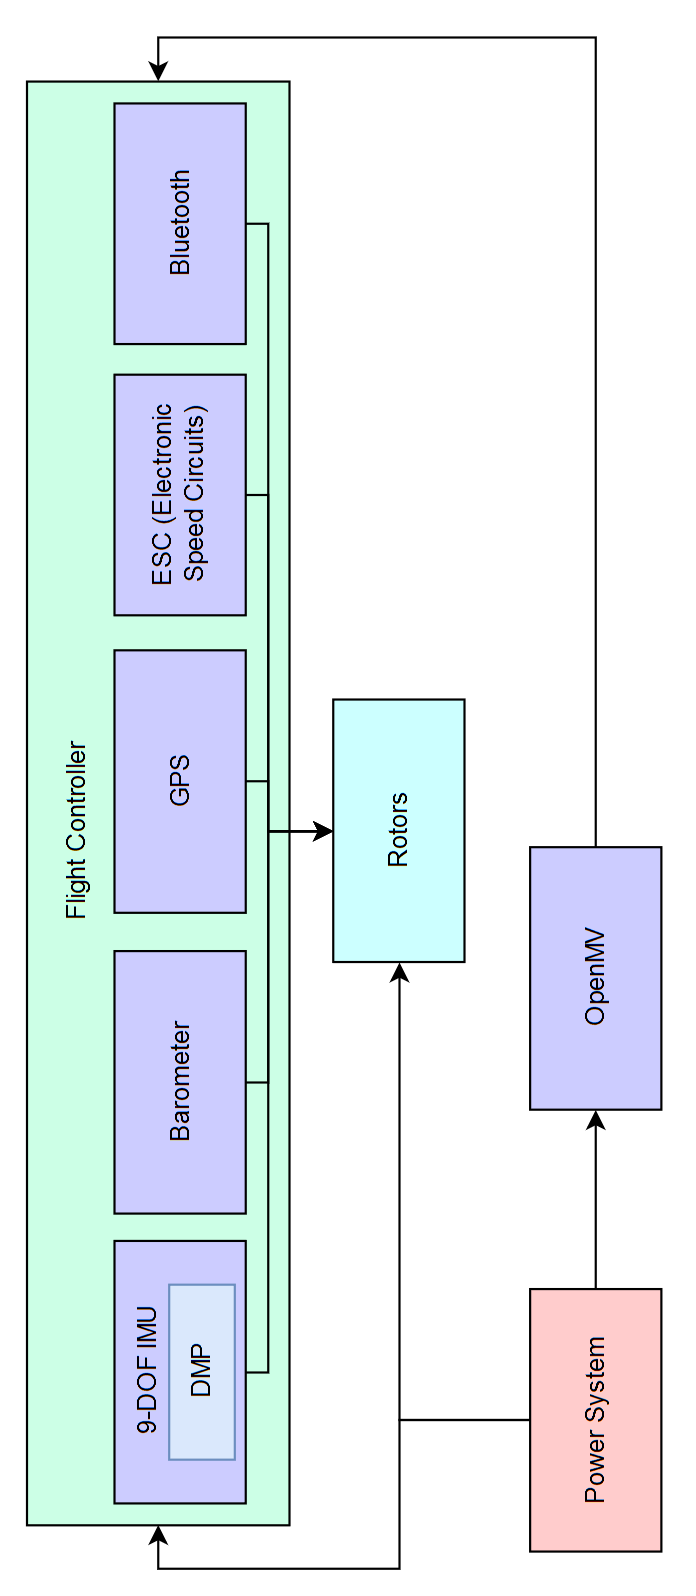
\includegraphics[width=0.95\textwidth]{child}
		\captionof{figure}{Block Diagram of Child Drone}
		\label{fig:child}
	\end{minipage}%
	\begin{minipage}[b]{0.5\textwidth}
		\centering
		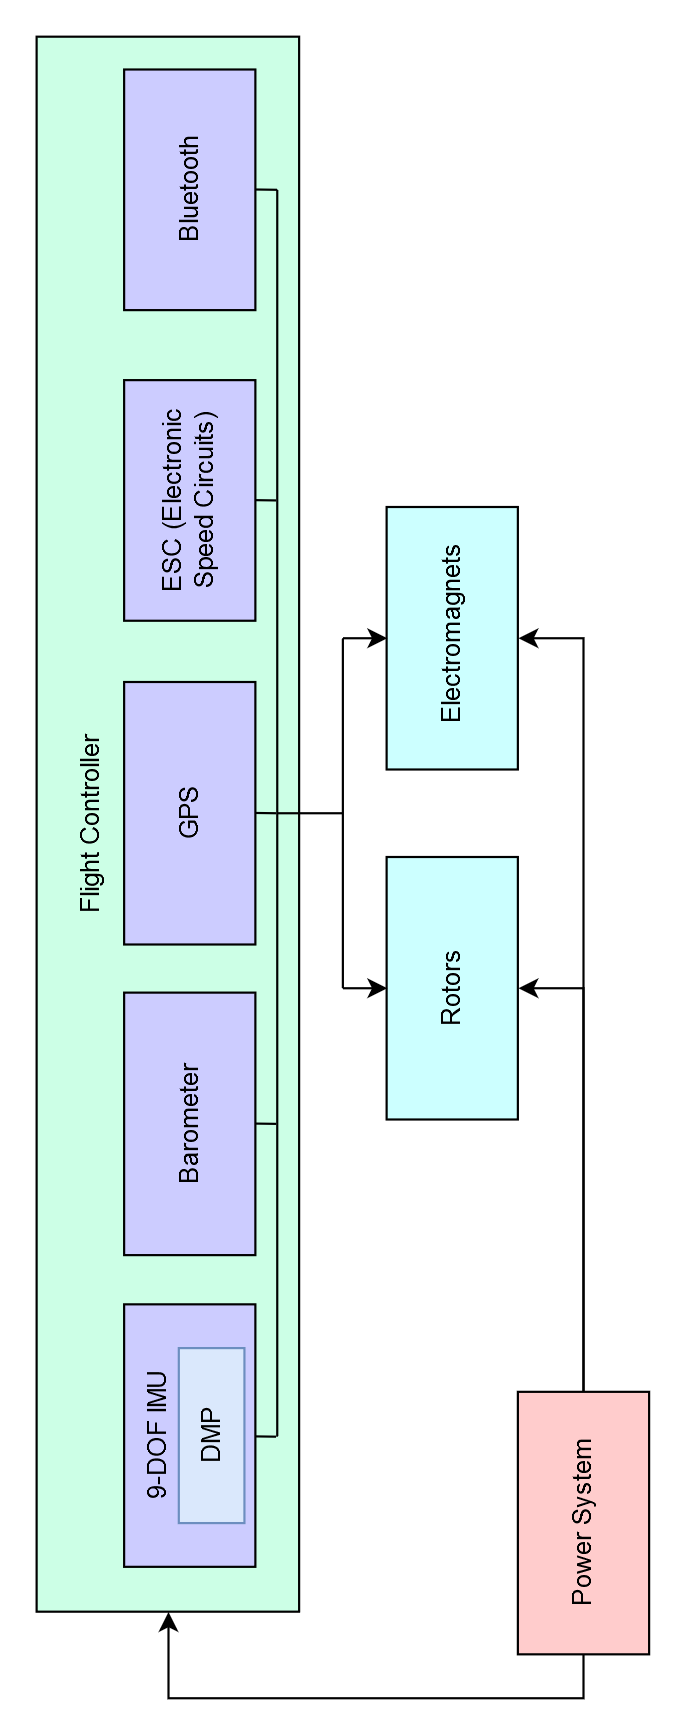
\includegraphics[width=0.95\textwidth]{parent}
		\captionof{figure}{Block Diagram of Parent Drone}
		\label{fig:parent}
	\end{minipage}
\end{figure}

\section{External Behavioral Specification}
Our project consists of two drones - a larger Parent drone and a smaller Child drone, hereinafter "Parent" and "Child". The Parent switches the battery of the Child while it is still flying. We listed the behavioral specifications of our project in the order that our demo is expected to go.
\begin{enumerate}
	\item The Parent carries a spare battery that will replace the Child's battery. The Child carries two batteries - one battery is the Child's main source of power while the other is an auxiliary power source for keeping the Child powered during the battery switch.  
	\item The Parent will fly to a height of 10 ft. and stabilize its position using a combination of signals from the 9 Degree-of-Freedom IMU and the barometer.
	\item The Parent has a GPS module, so it will send its location to our mobile app via Bluetooth. The mobile app will send the Parent's location to the Child via Wifi.
	\item The Child will fly towards the Parent using its own GPS module. In addition, the Child will fly an additional 5 ft. above the received Parent's height.
	\item The Child's OpenMV camera will search for an AprilTag that is printed and visible on the upper mount of the Parent's chassis. Once the Child  locates the Parent and determines its orientation with respect to the Parent, it will align itself directly over the Parent and descend directly downwards.
	\item Once the Child is close enough to the Parent , it will lower its rotors' speed and latch onto the Parent. The Parent has four poles on its top side, with two electromagnets located on a set of two poles that are diagonally opposite from each other. The Child has magnets on its underside that are aligned with the location of the electromagnets on the poles. Latching is complete when the two drones are held together by the magnets. 
	\item Once latching is complete, the Child's propellers will stop spinning and the Parent will carry the Child entirely. The Parent will re-stabilize itself after the entire latching process with the help of the DJI Naza-M V2 flight controller.
	\item The Child's batteries are hooked up in parallel (for seamless battery switching while keeping the Child powered through the auxiliary battery). The boxes that contain the batteries are connected to the underside of the Child drone. The batteries can be moved by sliding them in one direction -- if we slide a new battery into the compartment from one side, the old battery will slide out of the compartment on the other end, effectively completing a battery switch. The Parent has two horizontally-sliding rods that will change the batteries in this manner.
	\item The "dead" battery will be secured to the Parent by attaching itself to the rod when it pushed out of the compartment. After the switch is complete, a servo latch to secure them in place, to prevent them from sliding out during flight. 
	\item After the new batteries are secured, the Child will begin to spin its propellers again. The Child will also send a signal to the Parent indicating that it wants to unlatch. When the Parent receives this signal, it reverses the polarity of the electromagnets, repelling the Child.
	\item After the Child unlatches, it can fly freely and resume what it was doing before its battery depleted.
\end{enumerate}

\section{Member Responsibilities}
The responsibilities of each member are given in Table \ref{table:responsibilities}. \\%
\\%
\underline{Battery Switching} is a task that two members will work on because it is a large task that has many small parts that must be done. Specifically, this task requires designing the compartments that will hold and secure the batteries. In addition, this task will require some 3D printing for the parts that will be involved in the battery switching. \\%
\\%
\underline{Parent \& Child Drone Construction} is another task that two members will work on. For this project, we are building both the Parent and Child drones from scratch. The construction itself will take a substantial amount of time, but this task also requires a lot of testing to ensure stable flight, which is integral for our project. In addition, this task also includes integration of sensors, peripherals, and other custom parts that we will design for this project.
\vspace{10pt}
\begin{table}[h!]
	\centering
	\begin{tabular}{|l|l|} 
		\hline
		\textbf{Name} & \textbf{Responsibilities} \\%
		\hline
		\hline
		Richard Boone & Electromagnetic Latching System, Battery Switching \\%
		\hline
		Kyle Douglas & Parent \& Child Drone Construction \\%
		\hline
		Sayali Kakade & Camera Latency Measurement, Image Recognition \\%
		\hline
		Sang Min Oh & Parent \& Child Drone Construction \\%
		\hline
		Aditya Wadaskar & On-Board Development with DJI's SDK, Battery Switching \\%
		\hline
	\end{tabular}
	\caption{Group Member Responsibilities}
	\label{table:responsibilities}
\end{table}

%%%%%%%%%%%%% END DOCUMENT CONTENT %%%%%%%%%%%%%

%%%%%%%%%%%%%%% BEGIN REFERENCES %%%%%%%%%%%%%%%

%%%%%%%%%%%%%%%% END REFERENCES %%%%%%%%%%%%%%%%

% End document
\end{document}